\chapter{Preventivo}
Di seguito viene riportato il preventivo per il progetto MegAlexa; esso si divide,per ogni periodo,in:
\begin{itemize}
	\item \textbf{Prospetto orario:} presenta la distribuzione oraria e la suddivisione nei ruoli per ogni membro del gruppo ZeroSeven;
	\item \textbf{Prospetto economico:}presenta le ore di impegno calcolate per i ruoli coinvolti ed il rispettivo costo;
\end{itemize}
La suddivisione oraria viene svolta avendo come riferimento le seguenti regole:
\begin{itemize}
	\item Ogni membro del gruppo deve coprire ogni ruolo almeno una volta durante il ciclo di sviluppo del prodotto;
	\item Il totale delle ore di lavoro dovrà essere equamente distribuito tra i membri;
	\item Non ci devono essere conflitti di interesse in cui un Verificatore debba controllare il proprio lavoro.
\end{itemize}
Le sigle utilizzate per i vari ruoli saranno:
\begin{itemize}
	\item \textbf{Re:} Responsabile di Progetto;
	\item \textbf{Am:} Amministratore;
	\item \textbf{An:} Analista;
	\item \textbf{Pt:} Progettista;
	\item \textbf{Pr:} Programmatore;
	\item \textbf{Ve:} Verificatore;
\end{itemize}

Per il preventivo si tiene conto che i periodi di Analisi dei Requisiti e di Analisi dei Requisiti di Dettaglio sono considerati di investimento del gruppo e  non a carico dei committente, per cui  le ore di impegno svolte durante questi non saranno conteggiate nelle ore totali da retribuire.

\newpage
\section{Analisi  dei Requisiti}
\subsection{Prospetto orario}
Il prospetto orario per il periodo di Analisi dei Requisiti è illustrato nella seguente tabella:

\begin{table}[ht]
	\begin{center}
		\rowcolors{1}{}{lightgray}
		\begin{tabular}{cccccccccccc}
			\rowcolor{coolblack}
			\hline 
			& \textcolor{white}{Nome} & \textcolor{white}{Re} & \textcolor{white}{Am} & \textcolor{white}{An} & \textcolor{white}{Pt} &\textcolor{white}{Pr} & \textcolor{white}{Ve} & \textcolor{white}{Totale} \\
			\hline
			
			&Mirko Franco          & 10 & - & 9 & - & - & 5 &24  \\
			&Bianca Ciuche        & -  & 6 & 10 & - & - & 8 & 24 \\
			&Stefano Zanatta     & 12& 8 & 4 & - & - & - & 24 \\
			&Andrea Deidda       &  -& 9 & 8 & - & - & 7 & 24 \\
			&Ludovico Brocca    & -& 4 & 9 & - & - & 11 & 24 \\
			&Matteo Depascale  & -& 6& 10 & - & - & 8 & 24 \\
			&Gian Marco Bratzu & 7& 6 & 8 & - & - & 10 & 24 \\
			\hline
			&\textbf{Ore totali ruolo} & 22 & 39 & 58 & - & - & 49 & 168 \\
		\end{tabular}
		\caption{Prospetto Orario nel periodo di Analisi dei Requisiti}
	\end{center}
\end{table}

Il seguente grafico rappresenta la suddivisione oraria dei ruoli all'interno del gruppo:
\begin{figure}[!ht]
	\begin{center}
		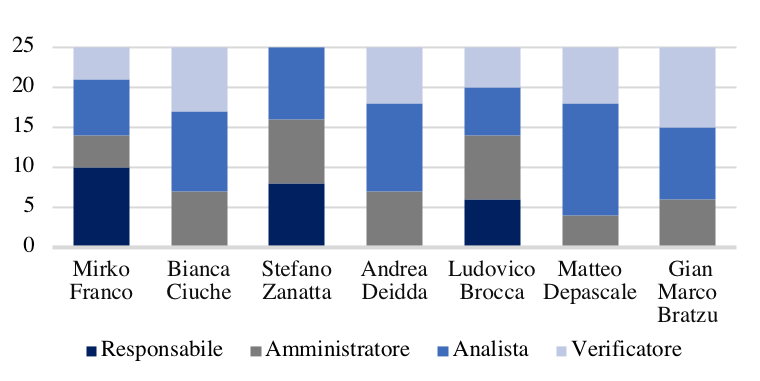
\includegraphics{images/grafoProspettoOrario.png}
		\caption{Grafico prospetto orario nel periodo di Analisi dei Requisiti }
	\end{center}
\end{figure}

\subsection{Prospetto Economico}
Il prospetto economico per il periodo di Analisi dei Requisiti è illustrato nella seguente tabella.
Le spese per questa attività non sono a carico del committente.

\begin{table}[ht]
	\begin{center}
		\rowcolors{1}{}{lightgray}
			\begin{tabular}{cccccc}
			\rowcolor{coolblack}
			\hline
			&\textcolor{white}{Ruolo}&	\textcolor{white}{Ore} &\textcolor{white}{Costo(\euro)} \\
			\hline
			&Responsabile           &22& 660  \\
			&Amministratore        & 39& 780 \\
			&Analista                   & 58& 1.450 \\
			&Progettista              &  -& - \\
			&Programmatore       & - & -  \\
			&Verificatore             & 49 & 735 \\
			\hline
			&\textbf{Ore totali}    &175& 3.845 \\
		\end{tabular}
		\caption{Prospetto Economico nel periodo di Analisi dei Requisiti}
	\end{center}
\end{table}

La raffigurazione grafica del peso di ogni ruolo sul costo totale è così rappresentata:
\begin{figure}[!ht]
	\centering
	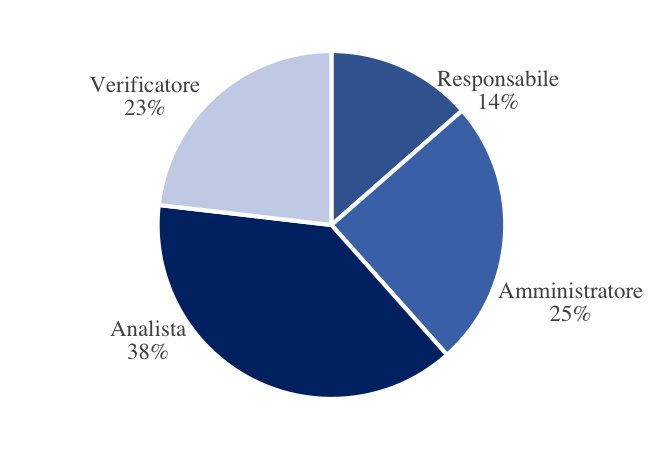
\includegraphics{images/grafoProspettoEconomico.png}
	\caption{Grafico prospetto economico nel periodo di Analisi dei Requisiti }
\end{figure}

\newpage
\section{Analisi dei Requisiti di Dettaglio}
\subsection{Prospetto Orario}
Il prospetto orario per il periodo di Analisi dei Requisiti di Dettaglio è illustrato nella seguente tabella:

\begin{table}[ht]
	\begin{center}
		\rowcolors{1}{}{lightgray}
		\begin{tabular}{cccccccccccc}
			\rowcolor{coolblack}
			\hline 
			& \textcolor{white}{Nome} & \textcolor{white}{Re} & \textcolor{white}{Am} & \textcolor{white}{An} & \textcolor{white}{Pt} &\textcolor{white}{Pr} & \textcolor{white}{Ve} & \textcolor{white}{Totale} \\
			\hline
			
			&Mirko Franco          & - & 3 & - & - & - & 2 &5  \\
			&Bianca Ciuche        & 5  & - & - & - & - & - & 5 \\
			&Stefano Zanatta     & -& - & 2 & - & - & 3&5 \\
			&Andrea Deidda       &  -& - & 2 & - & - & 3 &5 \\
			&Ludovico Brocca    & -& -& 3 & - & - & 2 & 5 \\
			&Matteo Depascale  & -& 2& -& - & - & 3 & 5 \\
			&Gian Marco Bratzu & -& - & 2 & - & - & 3& 5 \\
			\hline
			&\textbf{Ore totali ruolo} & 5 & 5 & 9 & - & - & 16 & 35 \\
		\end{tabular}
		\caption{Prospetto Orario nel periodo di Analisi dei Requisiti di Dettaglio}
	\end{center}
\end{table}

Il seguente grafico rapresenta la suddivisione oraria dei ruoli all'interno del gruppo:
\begin{figure}[!ht]
	\begin{center}
		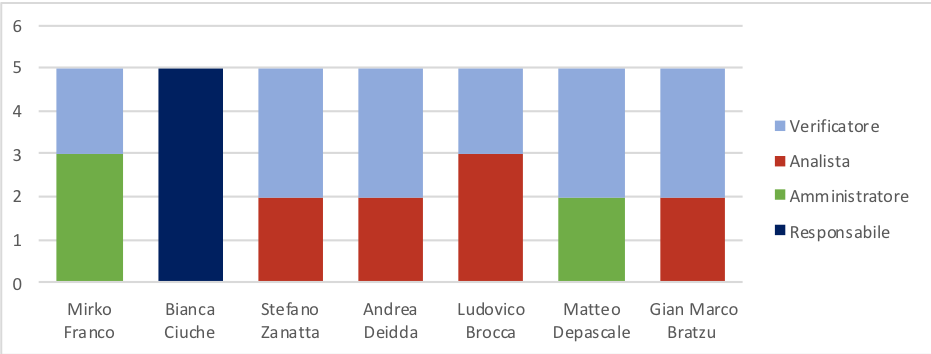
\includegraphics{images/grafoProspettoOrarioDett.png}
		\caption{Grafico prospetto orario nel periodo di Analisi dei Requisiti in Dettaglio}
	\end{center}
\end{figure}
\newpage
\subsection{Prospetto economico}
Il prospetto economico per il periodo di Analisi dei Requisiti di Dettaglio è illustrato nella seguente tabella.
Le spese per questa attività non sono a carico del committente.
\begin{table}[ht]
	\begin{center}
		\rowcolors{1}{}{lightgray}
		\begin{tabular}{cccccc}
			\rowcolor{coolblack}
			\hline
			&\textcolor{white}{Ruolo}&	\textcolor{white}{Ore} &\textcolor{white}{Costo(\euro)} \\
			\hline
			&Responsabile           &5&150  \\
			&Amministratore        & 5& 100 \\
			&Analista                   & 9& 225 \\
			&Progettista              &  -& - \\
			&Programmatore       & - & -  \\
			&Verificatore             & 11 & 165 \\
			\hline
			&\textbf{Ore totali}    &30& 640\\
		\end{tabular}
		\caption{Prospetto Economico nel periodo di Analisi dei Requisiti di Dettaglio}
	\end{center}
\end{table}

La raffigurazione grafica del peso di ogni ruolo sul costo totale è così rappresentata:
\begin{figure}[!ht]
	\begin{center}
		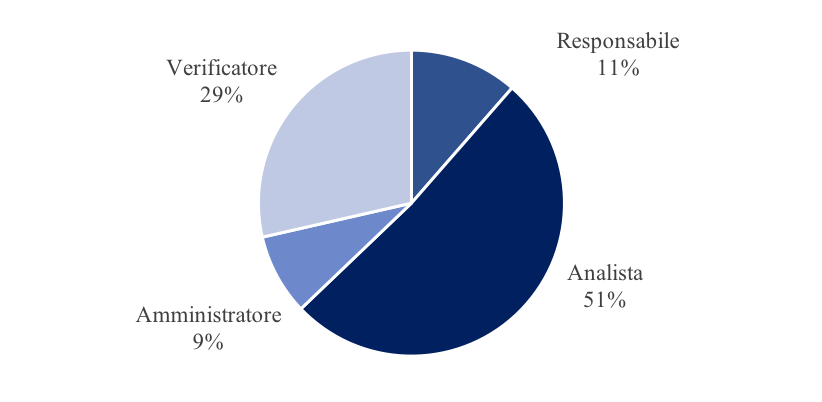
\includegraphics{images/grafoProspettoEconomicoDett.png}
		\caption{Grafico prospetto economico nel periodo di Analisi dei Requisiti in Dettaglio }
	\end{center}
\end{figure}

\newpage
\section{Progettazione della Base Tecnologica}
\subsection{Prospetto orario}
Il prospetto orario durante il periodo di Progettazione della Base Tecnologica è illustrato nella seguente tabella:

\begin{table}[ht]
	\begin{center}
		\rowcolors{1}{}{lightgray}
		\begin{tabular}{ccccccccc}
			\rowcolor{coolblack}
			\hline
			& \textcolor{white}{Nome} & \textcolor{white}{Re} & \textcolor{white}{Am} & \textcolor{white}{An} & \textcolor{white}{Pt} &\textcolor{white}{Pr} & \textcolor{white}{Ve} & \textcolor{white}{Totale} \\
			\hline
			&Mirko Franco & - & 5 & 9 & 9 & 6 & - & 29  \\
			&Bianca Ciuche & -& - & 6 & 10 & - & 11 & 27 \\
			&Stefano Zanatta & 5 & - & - & 22 & - & - & 27 \\
			&Andrea Deidda &  -& - & - & 12 & 4 & 13 & 29 \\
			&Ludovico Brocca & -& 5 & - & 19 & 5 & - & 29 \\
			&Matteo Depascale & -& - & - & 11 & - & 18 & 29 \\
			&Gian Marco Bratzu & 7& - & - & 20 & - & - & 27 \\
			\hline
			&\textbf{Ore totali ruolo} & 12 & 10 & 15 & 103 & 15 & 42 & 197 \\
		\end{tabular}
		\caption{Prospetto Orario nel periodo di Progettazione della Base Tecnologica}
	\end{center}
\end{table}

Il seguente grafico rapresenta la suddivisione oraria dei ruoli all'interno del gruppo:
\begin{figure}[!ht]
	\begin{center}
		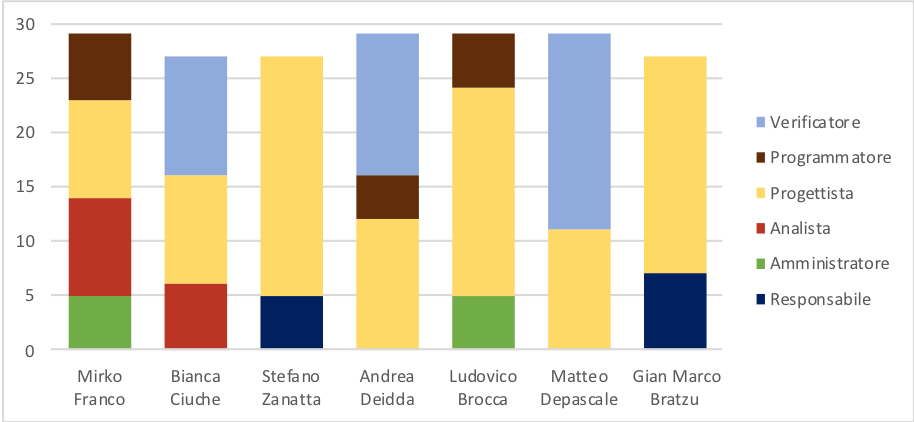
\includegraphics[scale=0.80]{images/grafoProgettazioneTecnologica.png}
		\caption{Grafico prospetto economico nel periodo di Progettazione della Base Tecnologica}
	\end{center}
\end{figure}
\newpage
\subsection{Prospetto economico}
Il prospetto economico per il periodo di Progettazione della Base Tecnologica è illustrato nella seguente tabella:

\begin{table}[ht]
	\begin{center}
		\rowcolors{1}{}{lightgray}
		\begin{tabular}{cccccc}
			\rowcolor{coolblack}
			\hline
			&\textcolor{white}{Ruolo}&	\textcolor{white}{Ore} &\textcolor{white}{Costo(\euro)} \\
			\hline
			&Responsabile           &12&360 \\
			&Amministratore        & 10& 200 \\
			&Analista                   & 15& 375 \\
			&Progettista              &  103& 2.266\\
			&Programmatore       & 15& 225 \\
			&Verificatore             & 42& 630 \\
			\hline
			&\textbf{Ore totali}    &197&4.056\\
		\end{tabular}
		\caption{Prospetto Economico nel periodo di Progettazione della Base Tecnologica}
	\end{center}
\end{table}


La raffigurazione grafica del peso di ogni ruolo sul costo totale è così rappresentata:
\begin{figure}[!ht]
	\begin{center}
		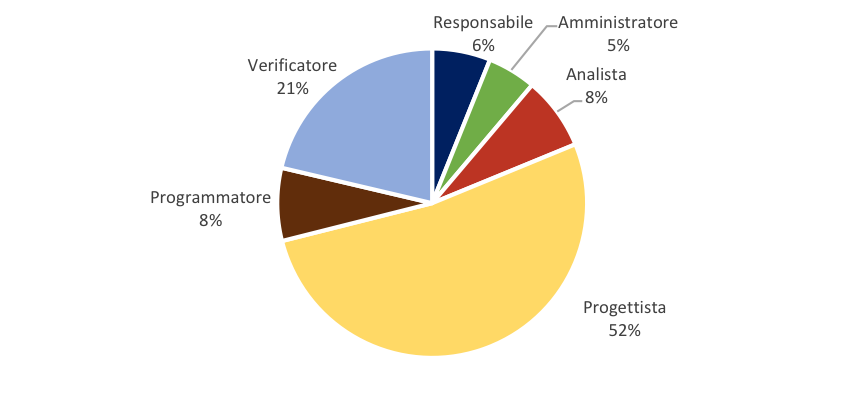
\includegraphics{images/grafoProgettazioneTecnologicaEuro.png}
		\caption{Grafico prospetto orario nel periodo di Analisi dei requisiti in dettaglio}
	\end{center}
\end{figure}
\newpage
\section{Progettazione di Dettaglio e Codifica}
\subsection{Prospetto orario}
Il prospetto orario durante il periodo di Progettazione di Dettaglio e Codifica è illustrato nella seguente tabella:

\begin{table}[ht]
	\begin{center}
		\rowcolors{1}{}{lightgray}
		\begin{tabular}{ccccccccc}
			\rowcolor{coolblack}
			\hline
			& \textcolor{white}{Nome} & \textcolor{white}{Re} & \textcolor{white}{Am} & \textcolor{white}{An} & \textcolor{white}{Pt} &\textcolor{white}{Pr} & \textcolor{white}{Ve} & \textcolor{white}{Totale} \\
			\hline
			&Mirko Franco & - & - & - & 8 & 22 & 21 & 51  \\
			&Bianca Ciuche & -& 6& - & 16 & 22 & 9 & 53 \\
			&Stefano Zanatta & - & - & 4 & 15 & 25 & 9 & 53 \\
			&Andrea Deidda &  -& - & 7 & 23 & 22 & - & 52 \\
			&Ludovico Brocca & 8& - & - & 13 & 18 & 11 & 50 \\
			&Matteo Depascale & -& 6& - & 20 & 14 & 12 & 52 \\
			&Gian Marco Bratzu & -& - & - & 22 & 21 & 10 & 53 \\
			\hline
			&\textbf{Ore totali ruolo} & 8 & 12 & 11 & 117 & 144 & 72 & 364 \\
		\end{tabular}
	\caption{Prospetto orario nel periodo di Progettazione di Dettaglio e Codifica}
	\end{center}
\end{table}

Il seguente grafico mostra una rappresentazione visiva della suddivisione oraria dei ruoli all'interno del gruppo:
\begin{figure}[!ht]
	\begin{center}
		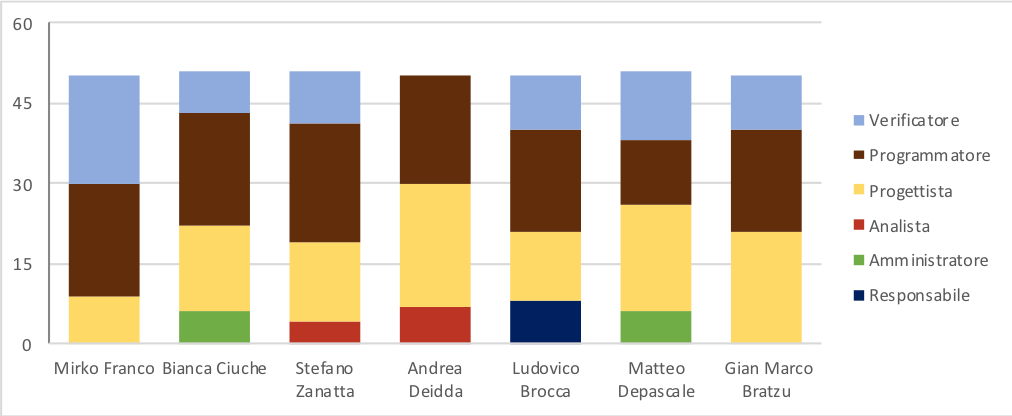
\includegraphics[scale=0.80]{images/grafoProgettazioneDettaglioCodifica.png}
		\caption{Grafico prospetto orario nel periodo di Progettazione di Dettaglio e Codifica}
	\end{center}
\end{figure}

\subsection{Prospetto economico}
Il prospetto economico durante il periodo di Progettazione di Dettaglio e Codifica è illustrato nella seguente tabella:

\begin{table}[ht]
	\begin{center}
		\rowcolors{1}{}{lightgray}
		\begin{tabular}{cccccc}
			\rowcolor{coolblack}
			\hline
			&\textcolor{white}{Ruolo}&	\textcolor{white}{Ore} &\textcolor{white}{Costo(\euro)} \\
			\hline
			&Responsabile           &8&240\\
			&Amministratore        & 12& 240 \\
			&Analista                   & 11& 275 \\
			&Progettista              &  117& 2.574\\
			&Programmatore       & 144& 2.160 \\
			&Verificatore             & 72& 1.080 \\
			\hline
			&\textbf{Ore totali}    &364&6.569\\
		\end{tabular}
		\caption{Prospetto Economico nel periodo di Progettazione di Dettaglio e Codifica}
	\end{center}
\end{table}

\begin{figure}[!ht]
	\begin{center}
		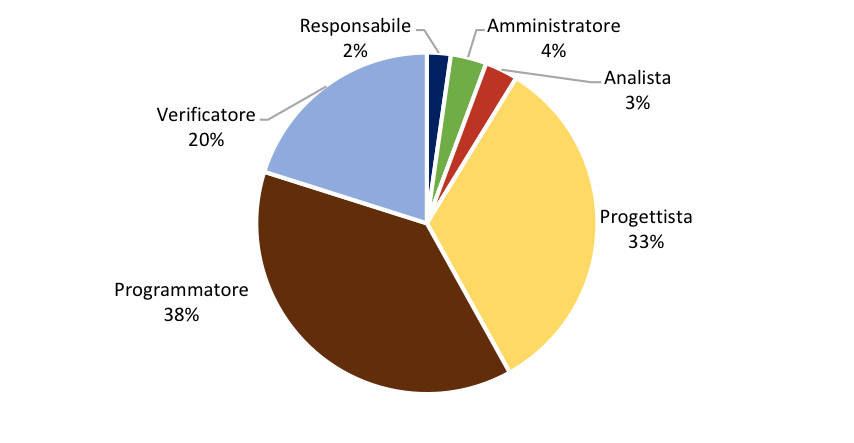
\includegraphics{images/grafoProgettazioneDettaglioCodificaEuro.png}
		\caption{Grafico prospetto economico nel periodo di Progettazione di Dettaglio e Codifica}
	\end{center}
\end{figure}

\newpage
\section{Validazione e Collaudo}
\subsection{Prospetto orario}
Il prospetto orario durante il periodo di Validazione e Collaudo è illustrato nella seguente tabella:

\begin{table}[ht]
	\begin{center}
		\rowcolors{1}{}{lightgray}
		\begin{tabular}{ccccccccc}
			\rowcolor{coolblack}
			\hline
			& \textcolor{white}{Nome} & \textcolor{white}{Re} & \textcolor{white}{Am} & \textcolor{white}{An} & \textcolor{white}{Pt} &\textcolor{white}{Pr} & \textcolor{white}{Ve} & \textcolor{white}{Totale} \\
			\hline
			&Mirko Franco & - & - & - & 9& - & 12 & 20  \\
			&Bianca Ciuche & -& -& - & 12 & - & 9 & 21 \\
			&Stefano Zanatta & - & 8& - & - & - & 13 & 21 \\
			&Andrea Deidda &  6& - & - & - & - & 14 & 20 \\
			&Ludovico Brocca & -& 9 & - & - & - & 13 & 22 \\
			&Matteo Depascale & 6& -& - & 3& 11& -& 20 \\
			&Gian Marco Bratzu & -& 4 & - & - & 14 & 3 & 21 \\
			\hline
			&\textbf{Ore totali ruolo} & 12& 21 & - & 24 & 25 & 64 & 145 \\
		\end{tabular}
		\caption{Prospetto orario nel periodo di Validazione e Collaudo}
	\end{center}
\end{table}

Il seguente grafico mostra una rappresentazione visiva della suddivisione oraria dei ruoli all'interno del gruppo:
\begin{figure}[!ht]
	\begin{center}
		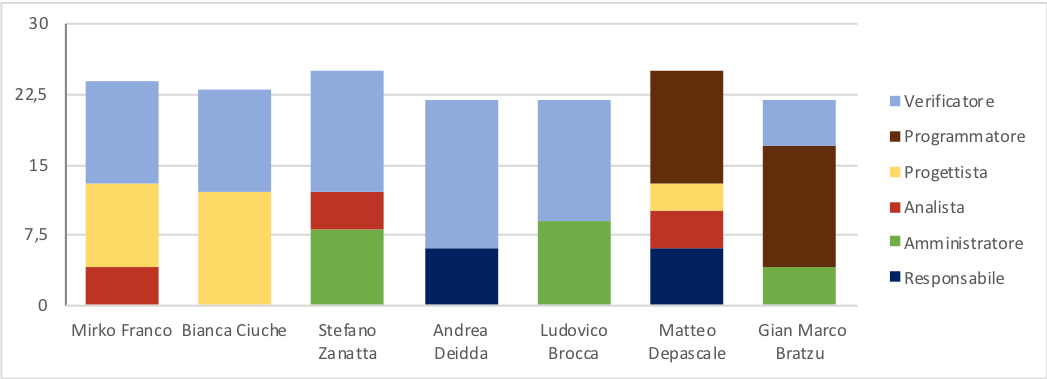
\includegraphics[scale=0.90]{images/grafoValidazioneCollaudo.png}
		\caption{Grafico prospetto orario nel periodo di Validazione e Collaudo}
	\end{center}
\end{figure}

\subsection{Prospetto economico}
Il prospetto economico durante il periodo di Validazione e Collaudo è illustrato nella seguente tabella:

\begin{table}[ht]
	\begin{center}
		\rowcolors{1}{}{lightgray}
		\begin{tabular}{cccccc}
			\rowcolor{coolblack}
			\hline
			&\textcolor{white}{Ruolo}&	\textcolor{white}{Ore} &\textcolor{white}{Costo(\euro)} \\
			\hline
			&Responsabile           &12&360\\
			&Amministratore        & 21& 420 \\
			&Analista                   & -& -\\
			&Progettista              &  24& 528\\
			&Programmatore       & 25& 375 \\
			&Verificatore             & 64& 960\\
			\hline
			&\textbf{Ore totali}    &146&2.643\\
		\end{tabular}
		\caption{Prospetto Economico nel periodo di Validazione e Collaudo}
	\end{center}
\end{table}

La raffigurazione grafica del peso di ogni ruolo sul costo totale è così rappresentata:
\begin{figure}[!ht]
	\begin{center}
		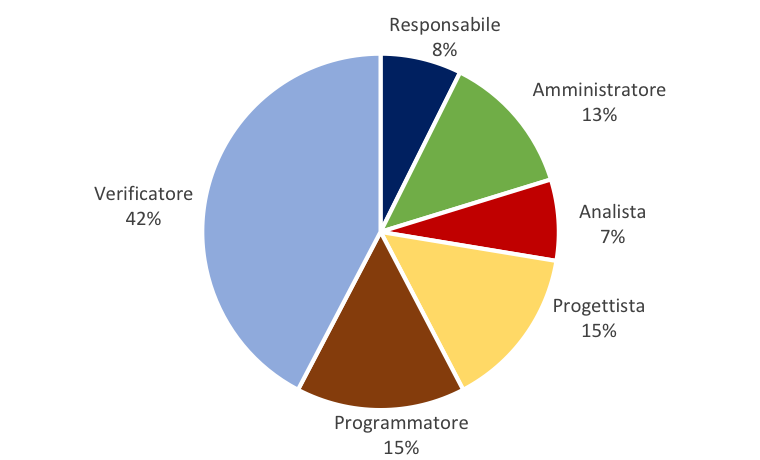
\includegraphics{images/grafoValidazioneCollaudoEuro.png}
		\caption{Grafico prospetto economico nel periodo di Validazione e Collaudo}
	\end{center}
\end{figure}
\newpage
\section{Totale ore rendicontate}
\subsection{Totale del  prospetto orario rendicontato}
Il totale del prospetto orario rendicontato è illustrato nella seguente tabella:

\begin{table}[ht]
	\begin{center}
		\rowcolors{1}{}{lightgray}
		\begin{tabular}{ccccccccc}
			\rowcolor{coolblack}
			\hline
			& \textcolor{white}{Nome} & \textcolor{white}{Re} & \textcolor{white}{Am} & \textcolor{white}{An} & \textcolor{white}{Pt} &\textcolor{white}{Pr} & \textcolor{white}{Ve} & \textcolor{white}{Totale} \\
			\hline
			&Mirko Franco & - & - & 14 & 26& 28 & 33 & 101  \\
			&Bianca Ciuche & -& 6& 6 & 38 & 22& 29 &101 \\
			&Stefano Zanatta & 5 & 8& 4 & 37 & 25 & 22 & 101 \\
			&Andrea Deidda &  6& - & 7 &35 & 26 & 27 & 101\\
			&Ludovico Brocca & 8& 14 & - & 32 & 23 & 24 & 101 \\
			&Matteo Depascale & 6& 6& - & 34& 25& 30& 101\\
			&Gian Marco Bratzu & 7& 4 & - & 42 & 35 & 13 &101 \\
			\hline
			&\textbf{Ore totali ruolo} & 32& 43 & 26 & 244 & 184 & 178 & 707 \\
		\end{tabular}
		\caption{Prospetto orario totale delle ore rendicontate}
	\end{center}
\end{table}


Il seguente grafico mostra una rappresentazione visiva della suddivisione oraria dei ruoli all'interno del gruppo:
\begin{figure}[!ht]
	\begin{center}
		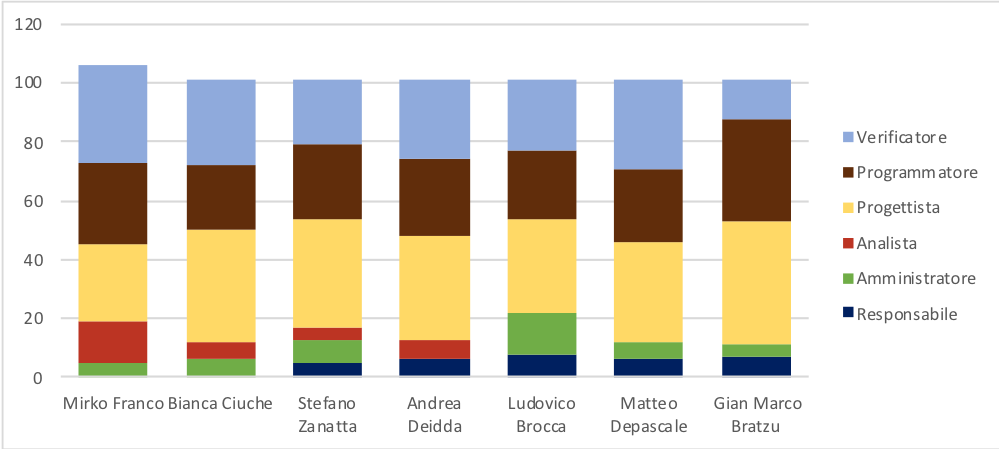
\includegraphics[scale=0.80]{images/grafoOreRendicontate.png}
		\caption{Grafico prospetto orario totale delle ore rendicontate}
	\end{center}
\end{figure}

\subsection{Totale del prospetto economico rendicontato}
La seguente tabella mostra il totale del prospetto economico rendicontato che  include le ore rendicontate nel preventivo a carico del committente cioè dei periodi di Progettazione della Base Tecnologica, Progettazione di Dettaglio e Codifica e il periodo di Validazione e Collaudo.

\begin{table}[ht]
	\begin{center}
		\rowcolors{1}{}{lightgray}
		\begin{tabular}{cccccc}
			\rowcolor{coolblack}
			\hline
			&\textcolor{white}{Ruolo}&	\textcolor{white}{Ore} &\textcolor{white}{Costo(\euro)} \\
			\hline
			&Responsabile           &32&960\\
			&Amministratore        & 43& 860 \\
			&Analista                   & 26& 650\\
			&Progettista              &  244& 5.368\\
			&Programmatore       & 184& 2.760 \\
			&Verificatore             & 178& 2.670\\
			\hline
			&\textbf{Ore totali}    &707&13.268\\
		\end{tabular}
		\caption{Prospetto economico totale delle ore rendicontate}
	\end{center}
\end{table}

La raffigurazione grafica del peso di ogni ruolo sul costo totale è così rappresentata:

\begin{figure}[!ht]
	\begin{center}
		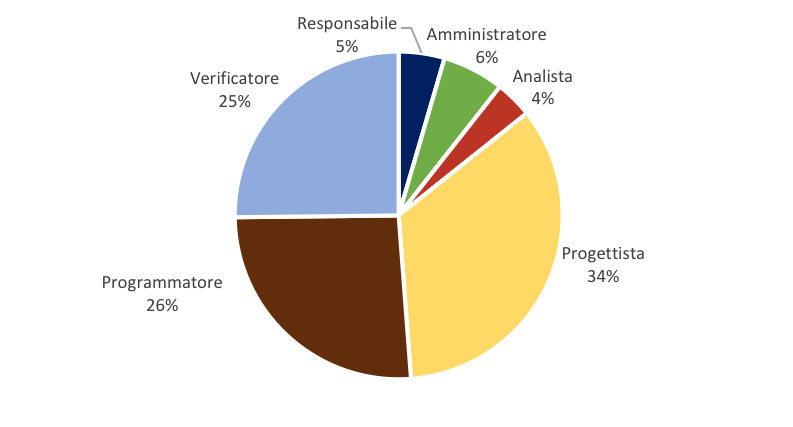
\includegraphics[scale=0.90]{images/grafoOreRendicontateEuro.png}
		\caption{Grafico prospetto economico totale delle ore rendicontate}
	\end{center}
\end{figure}

\section{Totale ore con investimento}
\subsection{Totale del prospetto orario con investimento}
Il totale del prospetto orario con investimento include sia le ore rendicontate nel preventivo a carico del committente sia le ore di investimento iniziali, esso è illustrato nella seguente tabella:

\begin{table}[ht]
	\begin{center}
		\rowcolors{1}{}{lightgray}
		\begin{tabular}{ccccccccc}
			\rowcolor{coolblack}
			\hline
			& \textcolor{white}{Nome} & \textcolor{white}{Re} & \textcolor{white}{Am} & \textcolor{white}{An} & \textcolor{white}{Pt} &\textcolor{white}{Pr} & \textcolor{white}{Ve} & \textcolor{white}{Totale} \\
			\hline
			&Mirko Franco & 10 & 8 & 18 & 26& 28 & 40 & 130  \\
			&Bianca Ciuche & 5& 12& 16& 38 & 22& 37 &130 \\
			&Stefano Zanatta & 17 & 16& 10 & 37 & 25 & 25 & 130\\
			&Andrea Deidda &  6& 9 & 17 &35 & 26 & 37 & 130\\
			&Ludovico Brocca & 8& 18 & 12 & 32 & 23 & 37 & 130 \\
			&Matteo Depascale & 6& 14& 10& 34& 25& 41& 130\\
			&Gian Marco Bratzu & 7& 10 & 10 & 42 & 35 & 26 &101 \\
			\hline
			&\textbf{Ore totali ruolo} & 59& 87 & 93 & 244 & 184 & 243 & 910 \\
		\end{tabular}
		\caption{Prospetto orario totale delle ore di investimento e rendicontate}
	\end{center}
\end{table}

Il seguente grafico mostra una rappresentazione visiva della suddivisione oraria dei ruoli all'interno del gruppo:
\begin{figure}[!ht]
	\begin{center}
		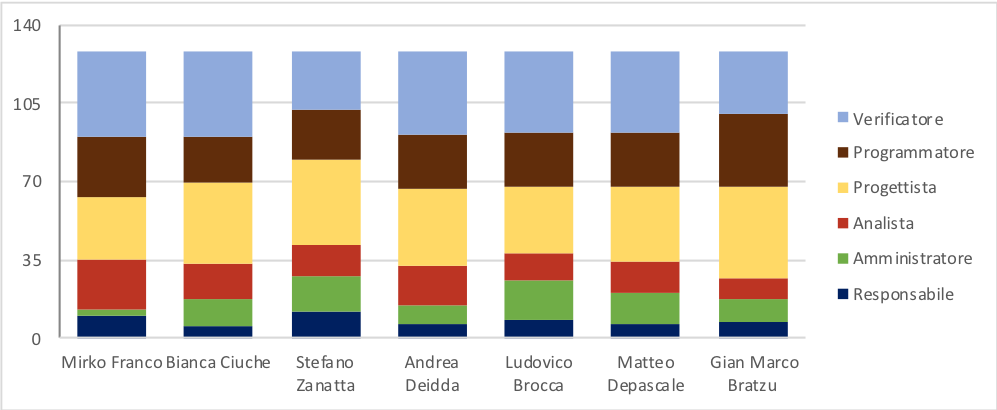
\includegraphics[scale=0.70]{images/grafoOreInvestimento.png}
		\caption{Grafico prospetto orario totale delle ore di investimento e rendicontate}
	\end{center}
\end{figure}
\newpage
\subsection{Totale del prospetto economico con investimento}
Il totale del prospetto economico con investimento include sia le ore rendicontate nel preventivo a carico del committente sia  le ore  di investimento iniziali, esso è illustrato nella seguente tabella:

\begin{table}[ht]
	\begin{center}
		\rowcolors{1}{}{lightgray}
		\begin{tabular}{cccccc}
			\rowcolor{coolblack}
			\hline
			&\textcolor{white}{Ruolo}&	\textcolor{white}{Ore} &\textcolor{white}{Costo(\euro)} \\
			\hline
			&Responsabile           &59&1.770\\
			&Amministratore        & 87& 1.740 \\
			&Analista                   & 93& 2.325\\
			&Progettista              &  244& 5.368\\
			&Programmatore       & 184& 2.760 \\
			&Verificatore             & 234& 3.645\\
			\hline
			&\textbf{Ore totali}    &910&17.608\\
		\end{tabular}
		\caption{Prospetto economico totale delle ore di investimento e rendicontate}
	\end{center}
\end{table}

La raffigurazione grafica del peso di ogni ruolo sul costo totale è così rappresentata:
\begin{figure}[!ht]
	\begin{center}
		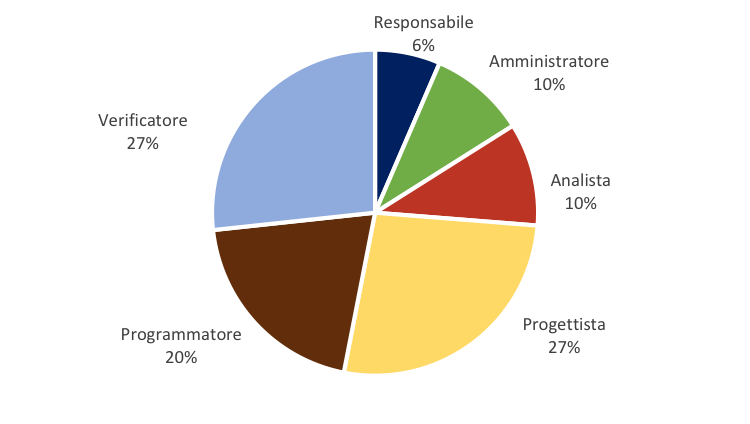
\includegraphics{images/grafoOreInvestimentoEuro.png}
		\caption{Grafico prospetto economico totale delle ore di investimento e rendicontate}
	\end{center}
\end{figure}



